\documentclass[11pt]{article}
\usepackage[textwidth=18.0cm, textheight=23.0cm, top=2.0cm]{geometry}
\usepackage{pst-all}
\usepackage{amssymb}
\usepackage{tikz}
\usepackage{underscore}\begin{document}
\pagestyle{empty}


ClassName: \underline{\textbf{Class_03.2bp-10}}
\par
BinSize: \underline{\textbf{40 × 40}}
\par
ReduceSize: \underline{\textbf{40 × 40}}
\par
TypeNum: \underline{\textbf{39}}
\par
Num: \underline{\textbf{40}}
\par
OutS: \underline{\textbf{9600}}
\par
InS: \underline{\textbf{8968}}
\par
Rate: \underline{\textbf{0.934}}
\par
UB: \underline{\textbf{6}}
\par
LB0: \underline{\textbf{6}}
\par
LB: \underline{\textbf{6}}
\par
LBWithCut: \underline{\textbf{6}}
\par
NodeCut: \underline{\textbf{0}}
\par
ExtendedNodeCnt: \underline{\textbf{1}}
\par
GenNodeCnt: \underline{\textbf{1}}
\par
PrimalNode: \underline{\textbf{4}}
\par
ColumnCount: \underline{\textbf{80}}
\par
TotalCutCount: \underline{\textbf{0}}
\par
RootCutCount: \underline{\textbf{0}}
\par
LPSolverCnt: \underline{\textbf{186}}
\par
PricingSolverCnt: \underline{\textbf{185}}
\par
BranchAndBoundNum: \underline{\textbf{1}}
\par
isOpt: \underline{\textbf{true}}
\par
TimeOnInitSolution: \underline{\textbf{0.015 s}}
\par
TimeOnPrimal: \underline{\textbf{864.400 s}}
\par
TimeOnPricing: \underline{\textbf{1167.050 s}}
\par
TimeOnRmp: \underline{\textbf{0.280 s}}
\par
TotalTime: \underline{\textbf{1167.672 s}}
\par
\newpage


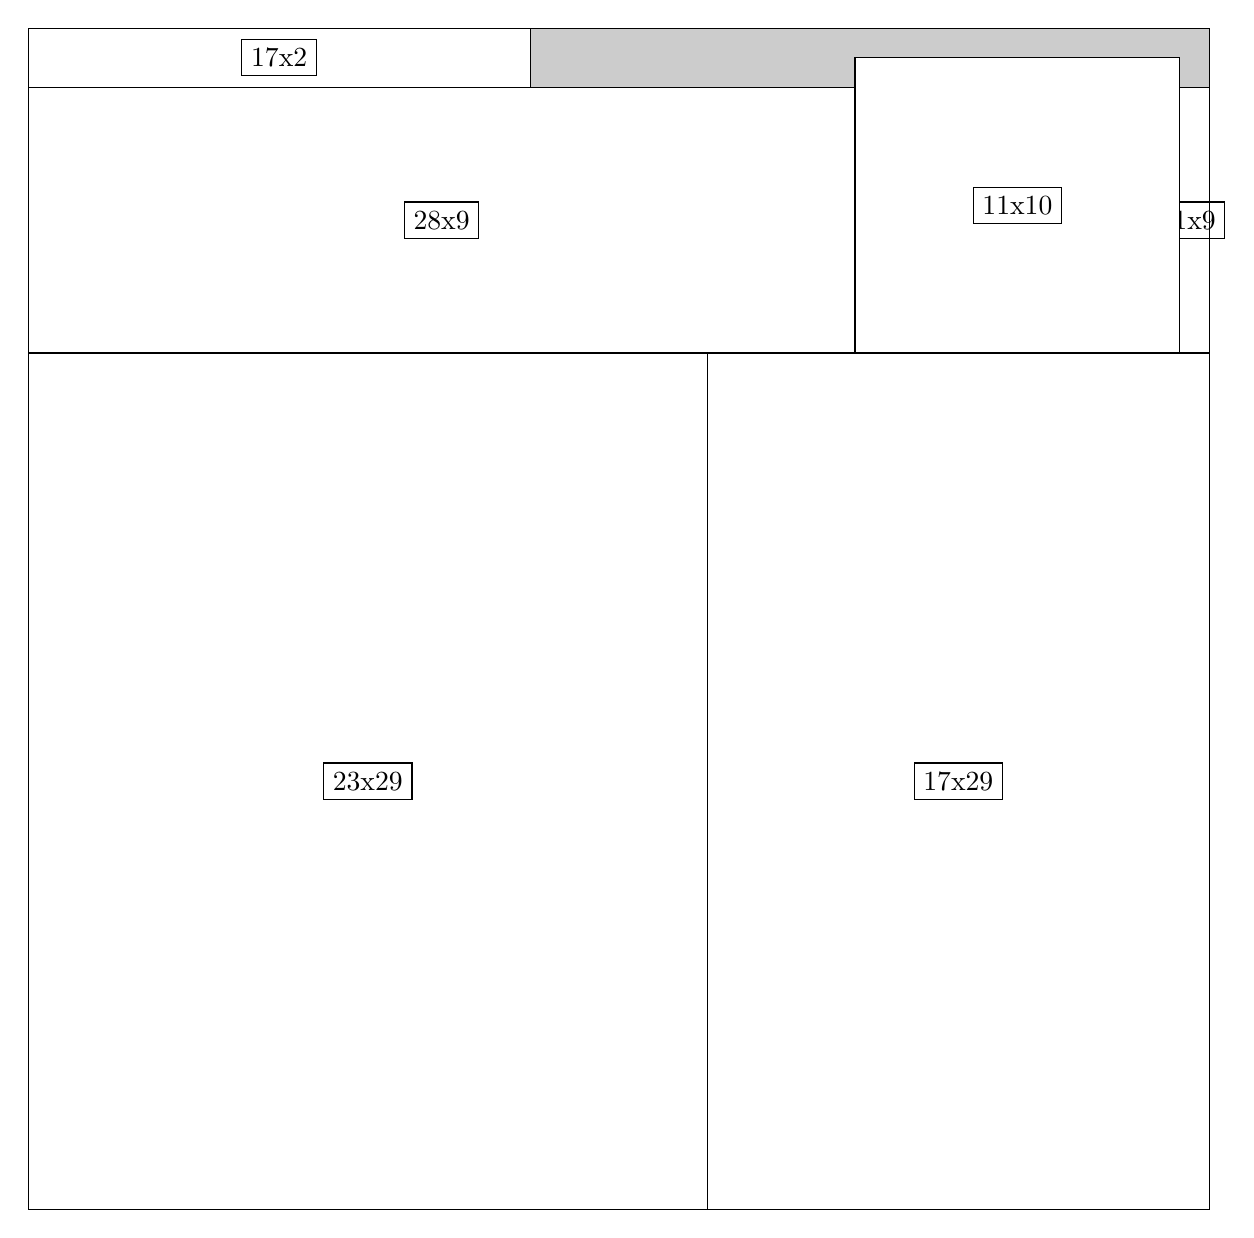
\begin{tikzpicture}[shorten >=1pt,scale=1.0,every node/.style={scale=1.0},->]
\tikzstyle{vertex}=[circle,fill=black!25,minimum size=14pt,inner sep=0pt]
\filldraw[fill=gray!40!white, draw=black] (0,0) rectangle (15.0,15.0);
\foreach \name/\x/\y/\w/\h in {17x2/0.0/14.25/6.375/0.75,1x9/14.625/10.875/0.375/3.375,11x10/10.5/10.875/4.125/3.75,28x9/0.0/10.875/10.5/3.375,17x29/8.625/0.0/6.375/10.875,23x29/0.0/0.0/8.625/10.875}
\filldraw[fill=white!40!white, draw=black] (\x,\y) rectangle node[draw] (\name) {\name} ++(\w,\h);
\end{tikzpicture}


w =17 , h =2 , x =0 , y =38 , v =34
\par
w =1 , h =9 , x =39 , y =29 , v =9
\par
w =11 , h =10 , x =28 , y =29 , v =110
\par
w =28 , h =9 , x =0 , y =29 , v =252
\par
w =17 , h =29 , x =23 , y =0 , v =493
\par
w =23 , h =29 , x =0 , y =0 , v =667
\par
\newpage


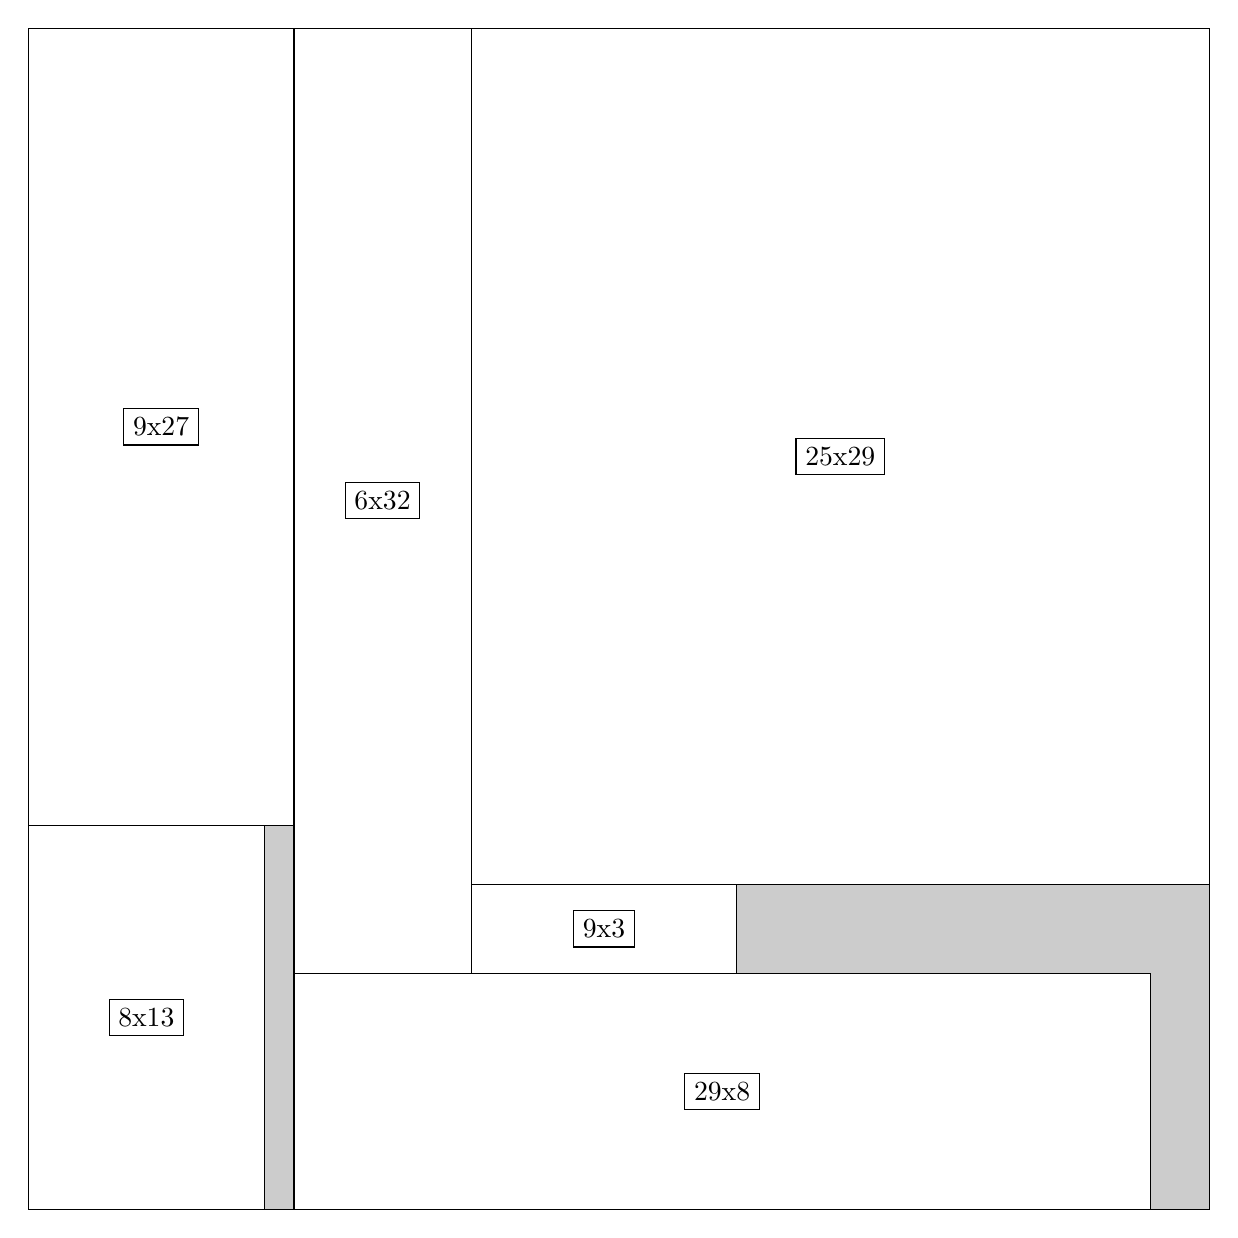
\begin{tikzpicture}[shorten >=1pt,scale=1.0,every node/.style={scale=1.0},->]
\tikzstyle{vertex}=[circle,fill=black!25,minimum size=14pt,inner sep=0pt]
\filldraw[fill=gray!40!white, draw=black] (0,0) rectangle (15.0,15.0);
\foreach \name/\x/\y/\w/\h in {8x13/0.0/0.0/3.0/4.875,9x27/0.0/4.875/3.375/10.125,29x8/3.375/0.0/10.875/3.0,6x32/3.375/3.0/2.25/12.0,9x3/5.625/3.0/3.375/1.125,25x29/5.625/4.125/9.375/10.875}
\filldraw[fill=white!40!white, draw=black] (\x,\y) rectangle node[draw] (\name) {\name} ++(\w,\h);
\end{tikzpicture}


w =8 , h =13 , x =0 , y =0 , v =104
\par
w =9 , h =27 , x =0 , y =13 , v =243
\par
w =29 , h =8 , x =9 , y =0 , v =232
\par
w =6 , h =32 , x =9 , y =8 , v =192
\par
w =9 , h =3 , x =15 , y =8 , v =27
\par
w =25 , h =29 , x =15 , y =11 , v =725
\par
\newpage


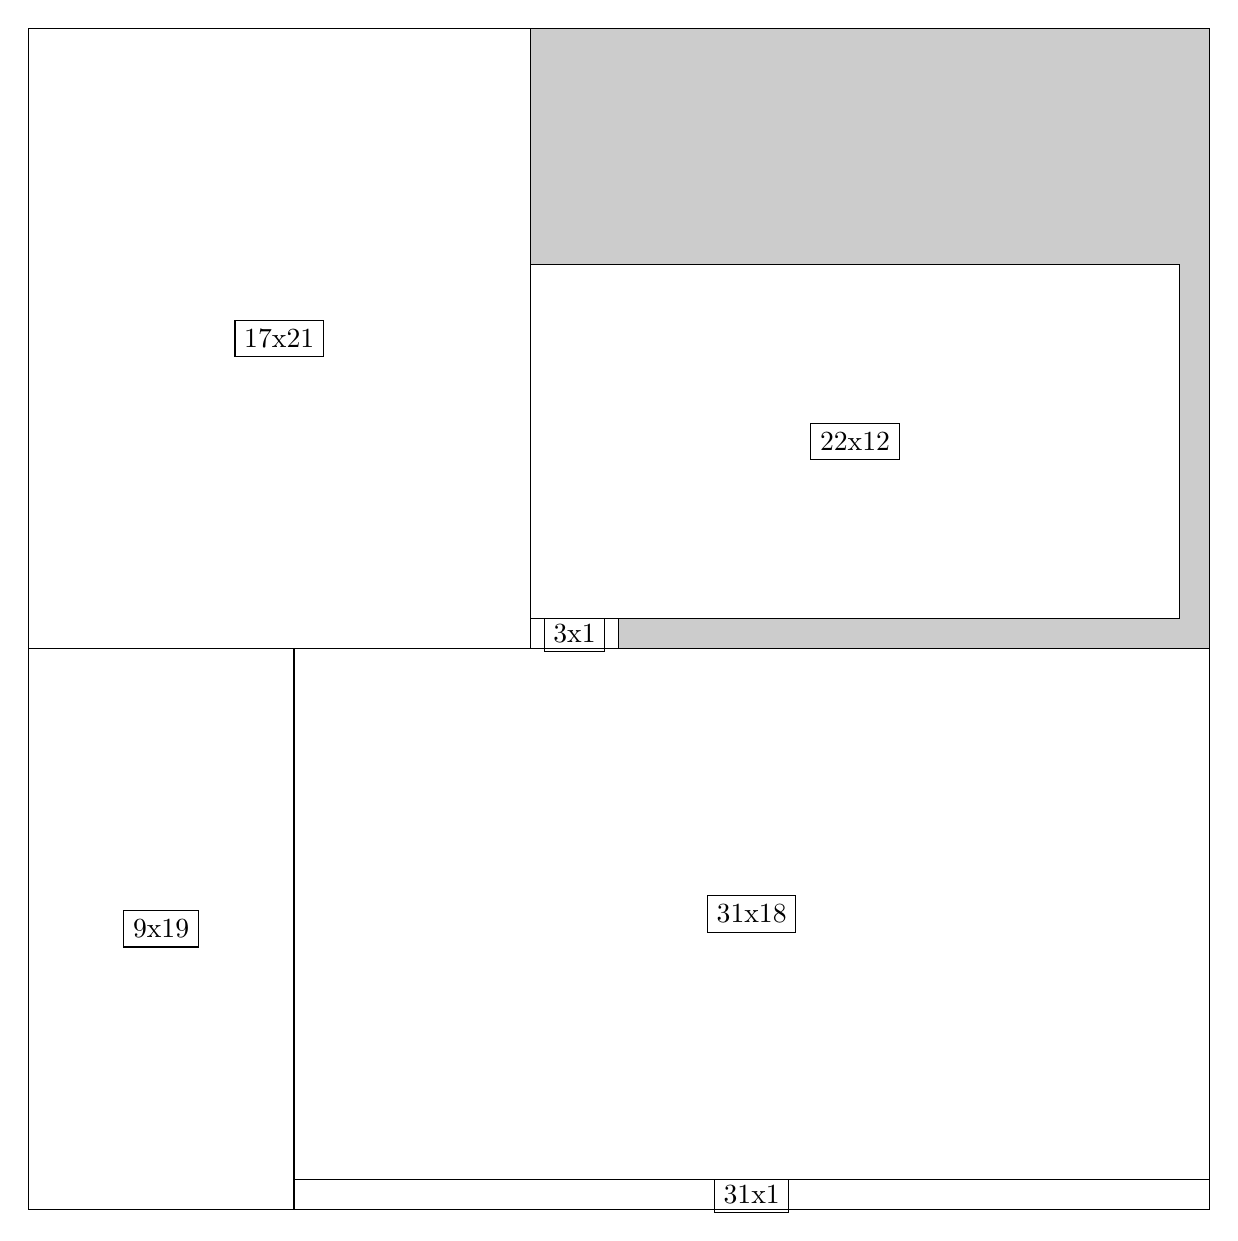
\begin{tikzpicture}[shorten >=1pt,scale=1.0,every node/.style={scale=1.0},->]
\tikzstyle{vertex}=[circle,fill=black!25,minimum size=14pt,inner sep=0pt]
\filldraw[fill=gray!40!white, draw=black] (0,0) rectangle (15.0,15.0);
\foreach \name/\x/\y/\w/\h in {9x19/0.0/0.0/3.375/7.125,31x1/3.375/0.0/11.625/0.375,31x18/3.375/0.375/11.625/6.75,17x21/0.0/7.125/6.375/7.875,3x1/6.375/7.125/1.125/0.375,22x12/6.375/7.5/8.25/4.5}
\filldraw[fill=white!40!white, draw=black] (\x,\y) rectangle node[draw] (\name) {\name} ++(\w,\h);
\end{tikzpicture}


w =9 , h =19 , x =0 , y =0 , v =171
\par
w =31 , h =1 , x =9 , y =0 , v =31
\par
w =31 , h =18 , x =9 , y =1 , v =558
\par
w =17 , h =21 , x =0 , y =19 , v =357
\par
w =3 , h =1 , x =17 , y =19 , v =3
\par
w =22 , h =12 , x =17 , y =20 , v =264
\par
\newpage


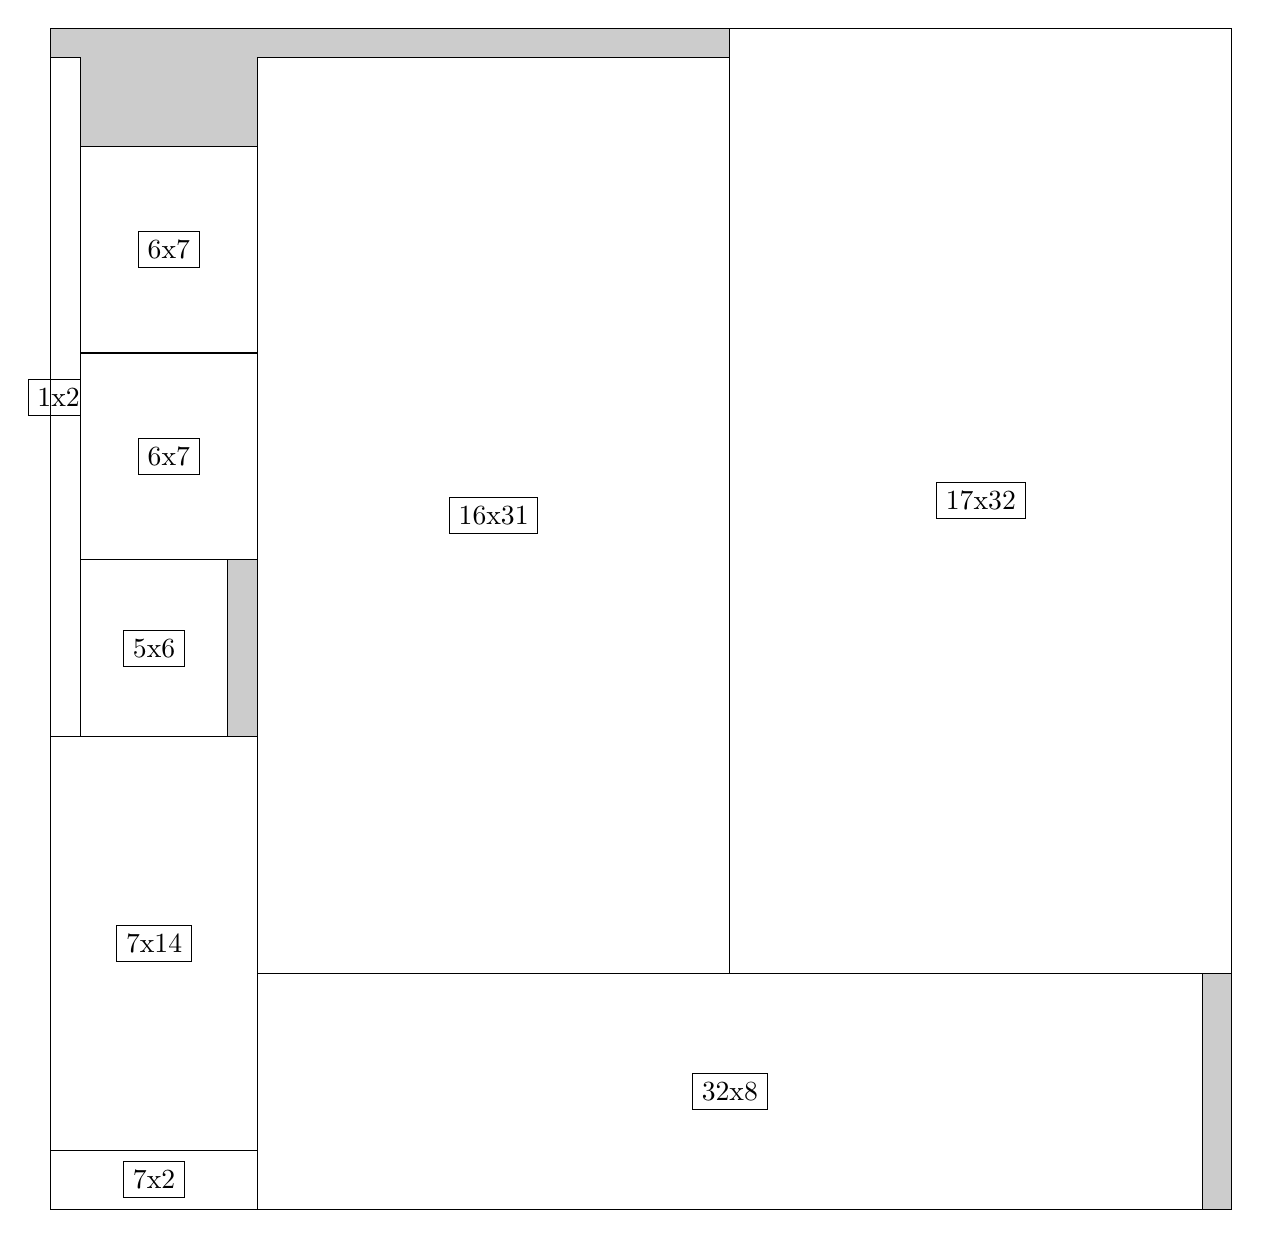
\begin{tikzpicture}[shorten >=1pt,scale=1.0,every node/.style={scale=1.0},->]
\tikzstyle{vertex}=[circle,fill=black!25,minimum size=14pt,inner sep=0pt]
\filldraw[fill=gray!40!white, draw=black] (0,0) rectangle (15.0,15.0);
\foreach \name/\x/\y/\w/\h in {7x2/0.0/0.0/2.625/0.75,7x14/0.0/0.75/2.625/5.25,1x23/0.0/6.0/0.375/8.625,5x6/0.375/6.0/1.875/2.25,6x7/0.375/8.25/2.25/2.625,6x7/0.375/10.875/2.25/2.625,32x8/2.625/0.0/12.0/3.0,16x31/2.625/3.0/6.0/11.625,17x32/8.625/3.0/6.375/12.0}
\filldraw[fill=white!40!white, draw=black] (\x,\y) rectangle node[draw] (\name) {\name} ++(\w,\h);
\end{tikzpicture}


w =7 , h =2 , x =0 , y =0 , v =14
\par
w =7 , h =14 , x =0 , y =2 , v =98
\par
w =1 , h =23 , x =0 , y =16 , v =23
\par
w =5 , h =6 , x =1 , y =16 , v =30
\par
w =6 , h =7 , x =1 , y =22 , v =42
\par
w =6 , h =7 , x =1 , y =29 , v =42
\par
w =32 , h =8 , x =7 , y =0 , v =256
\par
w =16 , h =31 , x =7 , y =8 , v =496
\par
w =17 , h =32 , x =23 , y =8 , v =544
\par
\newpage


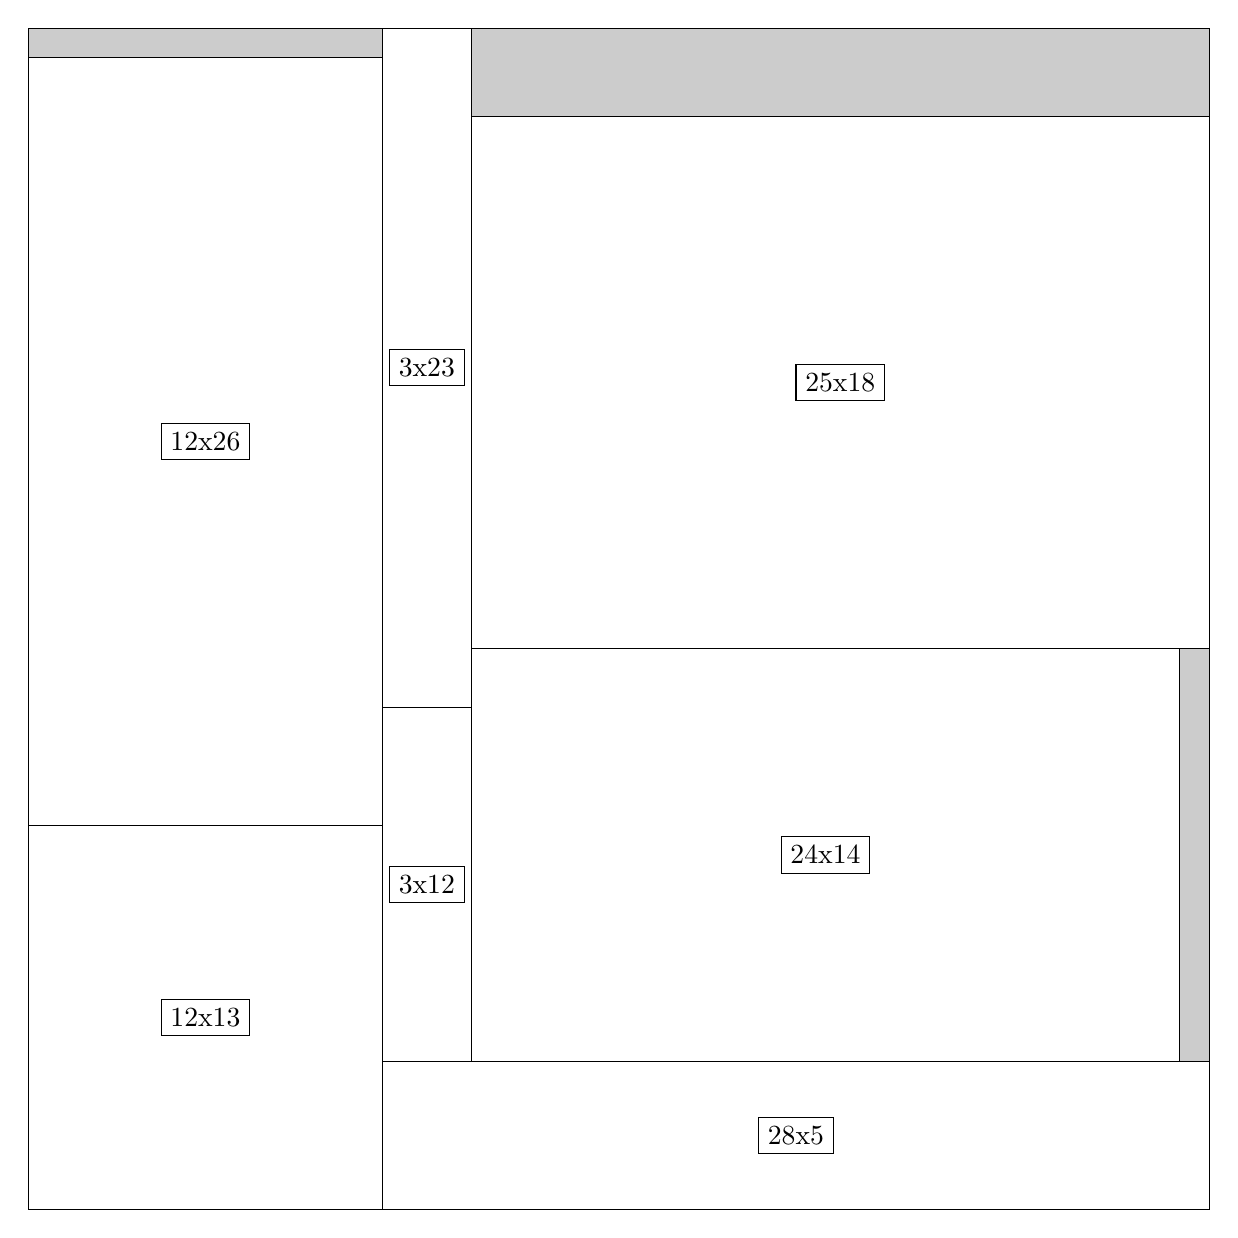
\begin{tikzpicture}[shorten >=1pt,scale=1.0,every node/.style={scale=1.0},->]
\tikzstyle{vertex}=[circle,fill=black!25,minimum size=14pt,inner sep=0pt]
\filldraw[fill=gray!40!white, draw=black] (0,0) rectangle (15.0,15.0);
\foreach \name/\x/\y/\w/\h in {12x13/0.0/0.0/4.5/4.875,12x26/0.0/4.875/4.5/9.75,28x5/4.5/0.0/10.5/1.875,3x12/4.5/1.875/1.125/4.5,3x23/4.5/6.375/1.125/8.625,24x14/5.625/1.875/9.0/5.25,25x18/5.625/7.125/9.375/6.75}
\filldraw[fill=white!40!white, draw=black] (\x,\y) rectangle node[draw] (\name) {\name} ++(\w,\h);
\end{tikzpicture}


w =12 , h =13 , x =0 , y =0 , v =156
\par
w =12 , h =26 , x =0 , y =13 , v =312
\par
w =28 , h =5 , x =12 , y =0 , v =140
\par
w =3 , h =12 , x =12 , y =5 , v =36
\par
w =3 , h =23 , x =12 , y =17 , v =69
\par
w =24 , h =14 , x =15 , y =5 , v =336
\par
w =25 , h =18 , x =15 , y =19 , v =450
\par
\newpage


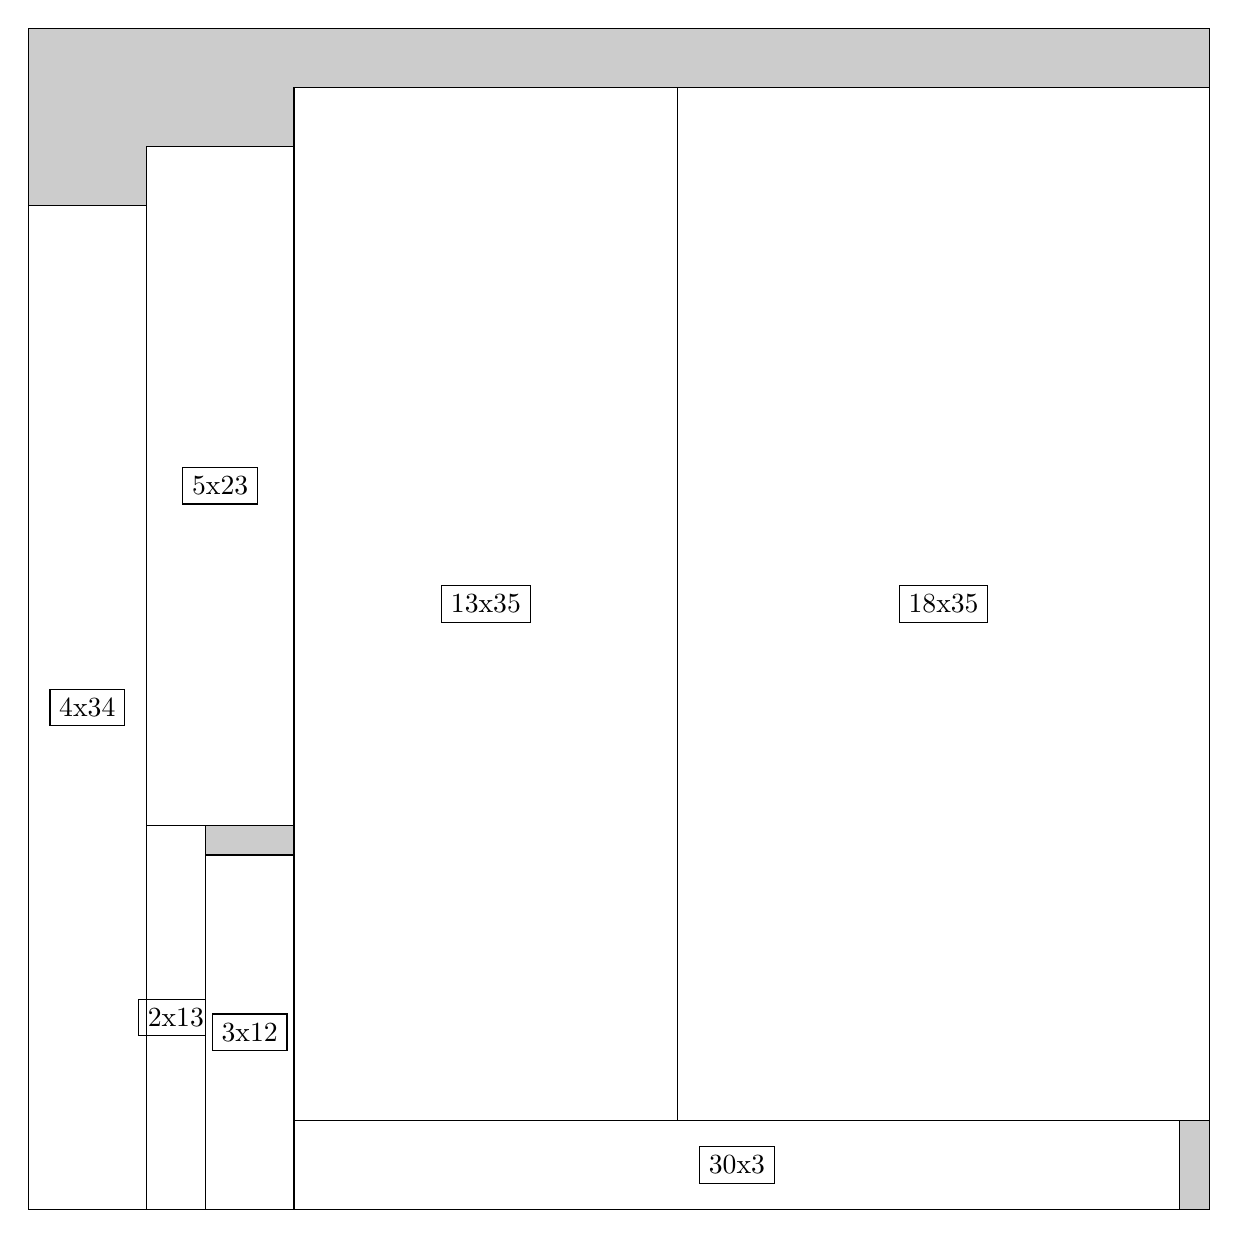
\begin{tikzpicture}[shorten >=1pt,scale=1.0,every node/.style={scale=1.0},->]
\tikzstyle{vertex}=[circle,fill=black!25,minimum size=14pt,inner sep=0pt]
\filldraw[fill=gray!40!white, draw=black] (0,0) rectangle (15.0,15.0);
\foreach \name/\x/\y/\w/\h in {4x34/0.0/0.0/1.5/12.75,2x13/1.5/0.0/0.75/4.875,3x12/2.25/0.0/1.125/4.5,5x23/1.5/4.875/1.875/8.625,30x3/3.375/0.0/11.25/1.125,13x35/3.375/1.125/4.875/13.125,18x35/8.25/1.125/6.75/13.125}
\filldraw[fill=white!40!white, draw=black] (\x,\y) rectangle node[draw] (\name) {\name} ++(\w,\h);
\end{tikzpicture}


w =4 , h =34 , x =0 , y =0 , v =136
\par
w =2 , h =13 , x =4 , y =0 , v =26
\par
w =3 , h =12 , x =6 , y =0 , v =36
\par
w =5 , h =23 , x =4 , y =13 , v =115
\par
w =30 , h =3 , x =9 , y =0 , v =90
\par
w =13 , h =35 , x =9 , y =3 , v =455
\par
w =18 , h =35 , x =22 , y =3 , v =630
\par
\newpage


\end{document}